Create a class that constructs and displays the following GUI: \\
%image is right-aligned to give students more writing space
\begin{minipage}{0.5\textwidth}
\vspace{-48pt}
The buttons within the GUI do not need to be functional.  You may or may not need the following: \texttt{JTextField}, \texttt{JButton}, \texttt{BorderLayout}, \texttt{BoxLayout}, \texttt{FlowLayout.LEFT}, \texttt{JFrame}, \texttt{JComponent}, \texttt{JDesktopPane}, and an exit-on-close operation.  The window should be 300 by 300 pixels and have a title.
\end{minipage}
\hspace{50px}
\begin{minipage}{0.3\textwidth}
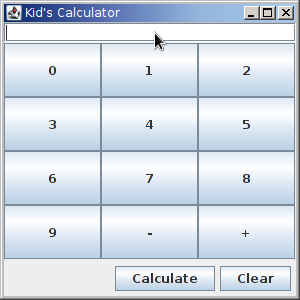
\includegraphics[scale=0.6]{other/calculator.png}
\end{minipage} \hfill

\vspace{-48pt}
\begin{answer}
\begin{lstlisting}[language=java,basicstyle=\small]
import java.awt.*;
import javax.swing.*;

public class BasicGUI {

	public BasicGUI() {
		JFrame frame = new JFrame("Kid's Calculator");
		frame.setLayout(new BorderLayout());
		
		JPanel top = new JPanel();
		top.setLayout(new BoxLayout(top, BoxLayout.LINE_AXIS));
		top.add(new JTextField());
		
		JPanel center = new JPanel();
		center.setLayout(new GridLayout(4,3));
		for(int i = 0; i < 10; ++i) {
			center.add(new JButton(Integer.toString(i)));
		}
		center.add(new JButton("-"));
		center.add(new JButton("+"));
		
		JPanel bottom = new JPanel();
		bottom.setLayout(new FlowLayout(FlowLayout.RIGHT));
		bottom.add(new JButton("Calculate"));
		JButton clearButton = new JButton("Clear");
		bottom.add(clearButton);
		
		Container pane = frame.getContentPane();
		pane.add(top, BorderLayout.NORTH);
		pane.add(center, BorderLayout.CENTER);
		pane.add(bottom, BorderLayout.SOUTH);
		
		frame.pack();
		frame.setSize(300, 300);
		frame.setDefaultCloseOperation(JFrame.EXIT_ON_CLOSE);
		frame.setVisible(true);
	}
	
	public static void main(String[] args) {
		BasicGUI gui = new BasicGUI();
	}
}
\end{lstlisting}
\end{answer}